\documentclass[]{article}
\usepackage{lmodern}
\usepackage{amssymb,amsmath}
\usepackage{ifxetex,ifluatex}
\usepackage{fixltx2e} % provides \textsubscript
\ifnum 0\ifxetex 1\fi\ifluatex 1\fi=0 % if pdftex
  \usepackage[T1]{fontenc}
  \usepackage[utf8]{inputenc}
\else % if luatex or xelatex
  \ifxetex
    \usepackage{mathspec}
  \else
    \usepackage{fontspec}
  \fi
  \defaultfontfeatures{Ligatures=TeX,Scale=MatchLowercase}
\fi
% use upquote if available, for straight quotes in verbatim environments
\IfFileExists{upquote.sty}{\usepackage{upquote}}{}
% use microtype if available
\IfFileExists{microtype.sty}{%
\usepackage{microtype}
\UseMicrotypeSet[protrusion]{basicmath} % disable protrusion for tt fonts
}{}
\usepackage[margin=1in]{geometry}
\usepackage{hyperref}
\hypersetup{unicode=true,
            pdftitle={Estadística II en R},
            pdfauthor={Fiona Franco Churruarín},
            pdfborder={0 0 0},
            breaklinks=true}
\urlstyle{same}  % don't use monospace font for urls
\usepackage{color}
\usepackage{fancyvrb}
\newcommand{\VerbBar}{|}
\newcommand{\VERB}{\Verb[commandchars=\\\{\}]}
\DefineVerbatimEnvironment{Highlighting}{Verbatim}{commandchars=\\\{\}}
% Add ',fontsize=\small' for more characters per line
\usepackage{framed}
\definecolor{shadecolor}{RGB}{248,248,248}
\newenvironment{Shaded}{\begin{snugshade}}{\end{snugshade}}
\newcommand{\AlertTok}[1]{\textcolor[rgb]{0.94,0.16,0.16}{#1}}
\newcommand{\AnnotationTok}[1]{\textcolor[rgb]{0.56,0.35,0.01}{\textbf{\textit{#1}}}}
\newcommand{\AttributeTok}[1]{\textcolor[rgb]{0.77,0.63,0.00}{#1}}
\newcommand{\BaseNTok}[1]{\textcolor[rgb]{0.00,0.00,0.81}{#1}}
\newcommand{\BuiltInTok}[1]{#1}
\newcommand{\CharTok}[1]{\textcolor[rgb]{0.31,0.60,0.02}{#1}}
\newcommand{\CommentTok}[1]{\textcolor[rgb]{0.56,0.35,0.01}{\textit{#1}}}
\newcommand{\CommentVarTok}[1]{\textcolor[rgb]{0.56,0.35,0.01}{\textbf{\textit{#1}}}}
\newcommand{\ConstantTok}[1]{\textcolor[rgb]{0.00,0.00,0.00}{#1}}
\newcommand{\ControlFlowTok}[1]{\textcolor[rgb]{0.13,0.29,0.53}{\textbf{#1}}}
\newcommand{\DataTypeTok}[1]{\textcolor[rgb]{0.13,0.29,0.53}{#1}}
\newcommand{\DecValTok}[1]{\textcolor[rgb]{0.00,0.00,0.81}{#1}}
\newcommand{\DocumentationTok}[1]{\textcolor[rgb]{0.56,0.35,0.01}{\textbf{\textit{#1}}}}
\newcommand{\ErrorTok}[1]{\textcolor[rgb]{0.64,0.00,0.00}{\textbf{#1}}}
\newcommand{\ExtensionTok}[1]{#1}
\newcommand{\FloatTok}[1]{\textcolor[rgb]{0.00,0.00,0.81}{#1}}
\newcommand{\FunctionTok}[1]{\textcolor[rgb]{0.00,0.00,0.00}{#1}}
\newcommand{\ImportTok}[1]{#1}
\newcommand{\InformationTok}[1]{\textcolor[rgb]{0.56,0.35,0.01}{\textbf{\textit{#1}}}}
\newcommand{\KeywordTok}[1]{\textcolor[rgb]{0.13,0.29,0.53}{\textbf{#1}}}
\newcommand{\NormalTok}[1]{#1}
\newcommand{\OperatorTok}[1]{\textcolor[rgb]{0.81,0.36,0.00}{\textbf{#1}}}
\newcommand{\OtherTok}[1]{\textcolor[rgb]{0.56,0.35,0.01}{#1}}
\newcommand{\PreprocessorTok}[1]{\textcolor[rgb]{0.56,0.35,0.01}{\textit{#1}}}
\newcommand{\RegionMarkerTok}[1]{#1}
\newcommand{\SpecialCharTok}[1]{\textcolor[rgb]{0.00,0.00,0.00}{#1}}
\newcommand{\SpecialStringTok}[1]{\textcolor[rgb]{0.31,0.60,0.02}{#1}}
\newcommand{\StringTok}[1]{\textcolor[rgb]{0.31,0.60,0.02}{#1}}
\newcommand{\VariableTok}[1]{\textcolor[rgb]{0.00,0.00,0.00}{#1}}
\newcommand{\VerbatimStringTok}[1]{\textcolor[rgb]{0.31,0.60,0.02}{#1}}
\newcommand{\WarningTok}[1]{\textcolor[rgb]{0.56,0.35,0.01}{\textbf{\textit{#1}}}}
\usepackage{graphicx,grffile}
\makeatletter
\def\maxwidth{\ifdim\Gin@nat@width>\linewidth\linewidth\else\Gin@nat@width\fi}
\def\maxheight{\ifdim\Gin@nat@height>\textheight\textheight\else\Gin@nat@height\fi}
\makeatother
% Scale images if necessary, so that they will not overflow the page
% margins by default, and it is still possible to overwrite the defaults
% using explicit options in \includegraphics[width, height, ...]{}
\setkeys{Gin}{width=\maxwidth,height=\maxheight,keepaspectratio}
\IfFileExists{parskip.sty}{%
\usepackage{parskip}
}{% else
\setlength{\parindent}{0pt}
\setlength{\parskip}{6pt plus 2pt minus 1pt}
}
\setlength{\emergencystretch}{3em}  % prevent overfull lines
\providecommand{\tightlist}{%
  \setlength{\itemsep}{0pt}\setlength{\parskip}{0pt}}
\setcounter{secnumdepth}{0}
% Redefines (sub)paragraphs to behave more like sections
\ifx\paragraph\undefined\else
\let\oldparagraph\paragraph
\renewcommand{\paragraph}[1]{\oldparagraph{#1}\mbox{}}
\fi
\ifx\subparagraph\undefined\else
\let\oldsubparagraph\subparagraph
\renewcommand{\subparagraph}[1]{\oldsubparagraph{#1}\mbox{}}
\fi

%%% Use protect on footnotes to avoid problems with footnotes in titles
\let\rmarkdownfootnote\footnote%
\def\footnote{\protect\rmarkdownfootnote}

%%% Change title format to be more compact
\usepackage{titling}

% Create subtitle command for use in maketitle
\providecommand{\subtitle}[1]{
  \posttitle{
    \begin{center}\large#1\end{center}
    }
}

\setlength{\droptitle}{-2em}

  \title{Estadística II en R}
    \pretitle{\vspace{\droptitle}\centering\huge}
  \posttitle{\par}
    \author{Fiona Franco Churruarín}
    \preauthor{\centering\large\emph}
  \postauthor{\par}
      \predate{\centering\large\emph}
  \postdate{\par}
    \date{30 December, 2019}


\begin{document}
\maketitle

{
\setcounter{tocdepth}{2}
\tableofcontents
}
\pagebreak

\hypertarget{probabilidad-y-variables-aleatorias}{%
\section{Probabilidad y Variables
Aleatorias}\label{probabilidad-y-variables-aleatorias}}

Una variable aleatoria le asgina un número cada elemento del espacio
muestral, es decir, a cada elemento del conjunto de todos los posibles
resultados de un experimento aleatorio.

\hypertarget{variables-aleatorias-y-sus-distribuciones}{%
\section{Variables aleatorias y sus
distribuciones}\label{variables-aleatorias-y-sus-distribuciones}}

Recordemos que una variable aleatoria (en adelante, v.a.) es discreta
cuando la imagen de \(x\) o su recorrido \(R_x\) es un conkunto finito o
infinito numerable, y que una v.a. es continua cuando su En esta sección
se verá como se implementan las distribuciones de probabilidad que se
utilizan en el curso. Es simple notar que todas las distribuciones
tienen un patron común en R.

Las v.a. discretas tienen asociada una \emph{función de probabilidad},
que devuelve la probabilidad \emph{puntual}, de que la variable
aleatoria \(x\) tome un determinado valor \(x_i\),

\[p(x_i) = p(x=x_i)\] Donde siempre se cumple que

\begin{enumerate}
\def\labelenumi{\arabic{enumi}.}
\item
  \(0 \leq p(x_i) \leq 1\)
\item
  \(\sum_{i=1}^n p(x_i)= 1\)
\end{enumerate}

Las v.a. aleatorias continuas tienen asociadas una \emph{función de
densidad}. Como el recorrido de la v.a. es continuo, no podemos
encontrar la probabilidad de ocurrencia de un sólo punto, es decir,
\(f(x=a)=0\) Para entender esto, recuérdese que no se puede calcular el
área bajo un sólo punto de una curva, porque es una sola linea. Por lo
tanto, se debe trabajar con la probabilidad de que la variable tome
valores entre dos puntos, para poder hallar el área debajo de la función
de densidad,

\[p(a \leq x \leq b) = \int_a^b f(x) dx.\]

En donde se cumple

\begin{enumerate}
\def\labelenumi{\arabic{enumi}.}
\item
  \(f(x) \geq 0\)
\item
  \(\int_{R_x} f(x) dx = 1\)
\end{enumerate}

Cada variable aleatoria también tiene una función de distribución
\(F(x)\)

\hypertarget{casos-discretos}{%
\subsection{Casos discretos}\label{casos-discretos}}

\hypertarget{distribucion-de-bernoulli}{%
\subsubsection{Distribución de
Bernoulli}\label{distribucion-de-bernoulli}}

\(x \sim Bern(p)\) Se utiliza para conocer la probabilidad de ocurrencia
de sucesos dicotómicos, es decir, aquellos en los que sólo hay dos
resultados posibles. Si llamamos \(x\) a la v.a., entonces podemos
denotar el espacio muestral de la variable de la siguiente forma,

\begin{equation}
x = 
\begin{cases} 
1 & \text{si } \mathrm{éxito} \\
0 & \text{si } \mathrm{fracaso}
\end{cases}
\end{equation}

Denominamos la probabilidad de ocurrencia del éxito \(p(x=1)\) como
\(p\), y la probabilidad de éxito del fracaso como \(1-p=q\). Así,
podemos escribir la función de probabilidad de una v.a. con distribución
de Bernoulli de la siguiente forma,

\[p(x) = p^x q^{1-x}\] En R esta distribución está codificadada con los
siguientes comandos

\begin{Shaded}
\begin{Highlighting}[]
\CommentTok{#dbinom(x, size, prob, log = FALSE)}
\CommentTok{#pbinom(q, size, prob, lower.tail = TRUE, log.p = FALSE)}
\CommentTok{#qbinom(p, size, prob, lower.tail = TRUE, log.p = FALSE)}
\CommentTok{#rbinom(n, size, prob)}


\KeywordTok{dbinom}\NormalTok{(}\DataTypeTok{x =} \DecValTok{1}\NormalTok{,   }\DataTypeTok{size =} \DecValTok{1}\NormalTok{, }\DataTypeTok{prob =} \FloatTok{0.5}\NormalTok{, }\DataTypeTok{log =} \OtherTok{FALSE}\NormalTok{)}
\end{Highlighting}
\end{Shaded}

\begin{verbatim}
## [1] 0.5
\end{verbatim}

\begin{Shaded}
\begin{Highlighting}[]
\KeywordTok{pbinom}\NormalTok{(}\DataTypeTok{q =} \DecValTok{1}\NormalTok{,   }\DataTypeTok{size =} \DecValTok{1}\NormalTok{, }\FloatTok{0.5}\NormalTok{, }\DataTypeTok{lower.tail =} \OtherTok{TRUE}\NormalTok{, }\DataTypeTok{log.p =} \OtherTok{FALSE}\NormalTok{)}
\end{Highlighting}
\end{Shaded}

\begin{verbatim}
## [1] 1
\end{verbatim}

\begin{Shaded}
\begin{Highlighting}[]
\KeywordTok{qbinom}\NormalTok{(}\DataTypeTok{p =} \FloatTok{0.5}\NormalTok{, }\DataTypeTok{size =} \DecValTok{1}\NormalTok{, }\FloatTok{0.5}\NormalTok{, }\DataTypeTok{lower.tail =} \OtherTok{TRUE}\NormalTok{, }\DataTypeTok{log.p =} \OtherTok{FALSE}\NormalTok{)}
\end{Highlighting}
\end{Shaded}

\begin{verbatim}
## [1] 0
\end{verbatim}

\begin{Shaded}
\begin{Highlighting}[]
\KeywordTok{rbinom}\NormalTok{(}\DataTypeTok{n =} \DecValTok{1}\NormalTok{,   }\DataTypeTok{size =} \DecValTok{1}\NormalTok{, }\FloatTok{0.5}\NormalTok{)}
\end{Highlighting}
\end{Shaded}

\begin{verbatim}
## [1] 1
\end{verbatim}

\hypertarget{distribucion-binomial}{%
\subsubsection{Distribución Binomial}\label{distribucion-binomial}}

Una v.a. \(x\) con distribución binomial, \(x \sim Bi(m,p)\), describe
el número de éxitos en \(m\) ensayos de Bernoulli independientes.

\[p(x) = \left(\begin{array}{l}{m} \\ {x}\end{array}\right) p^{x}q^{m-x}\]

\begin{Shaded}
\begin{Highlighting}[]
\NormalTok{m <-}\StringTok{ }\DecValTok{5}

\KeywordTok{dbinom}\NormalTok{(}\DataTypeTok{x =} \DecValTok{1}\NormalTok{,   }\DataTypeTok{size =}\NormalTok{ m, }\DataTypeTok{prob =} \FloatTok{0.5}\NormalTok{, }\DataTypeTok{log =} \OtherTok{FALSE}\NormalTok{)}
\end{Highlighting}
\end{Shaded}

\begin{verbatim}
## [1] 0.15625
\end{verbatim}

\begin{Shaded}
\begin{Highlighting}[]
\KeywordTok{pbinom}\NormalTok{(}\DataTypeTok{q =} \DecValTok{1}\NormalTok{,   }\DataTypeTok{size =}\NormalTok{ m, }\DataTypeTok{prob =} \FloatTok{0.5}\NormalTok{, }\DataTypeTok{lower.tail =} \OtherTok{TRUE}\NormalTok{, }\DataTypeTok{log.p =} \OtherTok{FALSE}\NormalTok{)}
\end{Highlighting}
\end{Shaded}

\begin{verbatim}
## [1] 0.1875
\end{verbatim}

\begin{Shaded}
\begin{Highlighting}[]
\KeywordTok{qbinom}\NormalTok{(}\DataTypeTok{p =} \FloatTok{0.5}\NormalTok{, }\DataTypeTok{size =}\NormalTok{ m, }\DataTypeTok{prob =} \FloatTok{0.5}\NormalTok{, }\DataTypeTok{lower.tail =} \OtherTok{TRUE}\NormalTok{, }\DataTypeTok{log.p =} \OtherTok{FALSE}\NormalTok{)}
\end{Highlighting}
\end{Shaded}

\begin{verbatim}
## [1] 2
\end{verbatim}

\begin{Shaded}
\begin{Highlighting}[]
\CommentTok{#rbinom(n = 1,   size = m, prob = 0.5,)}
\end{Highlighting}
\end{Shaded}

\hypertarget{distribucion-geometrica}{%
\subsubsection{Distribución geométrica}\label{distribucion-geometrica}}

\begin{Shaded}
\begin{Highlighting}[]
\CommentTok{#dgeom(x, prob, log = FALSE)}
\CommentTok{#pgeom(q, prob, lower.tail = TRUE, log.p = FALSE)}
\CommentTok{#qgeom(p, prob, lower.tail = TRUE, log.p = FALSE)}
\CommentTok{#rgeom(n, prob)}
\end{Highlighting}
\end{Shaded}

\(x \sim Ge(p)\) describe el número de ensayos de Bernoulli
independientes necesarios hasta obtener el primer éxito.

\[p(x) = pq^{x-1}\]

\hypertarget{distribucion-de-poisson}{%
\subsubsection{Distribución de Poisson}\label{distribucion-de-poisson}}

\(x \sim P(\lambda)\) describe el número de ocurrencias en un continuo
(tiempo, volúmen, etc). Se supone que la cantidad de ocurrencias es
directamente proporcional al continuo.

\[p(x) = \frac{e^{- \lambda} \lambda^x}{x!}\]

\begin{Shaded}
\begin{Highlighting}[]
\CommentTok{#dpois(x, lambda, log = FALSE)}
\CommentTok{#ppois(q, lambda, lower.tail = TRUE, log.p = FALSE)}
\CommentTok{#qpois(p, lambda, lower.tail = TRUE, log.p = FALSE)}
\CommentTok{#rpois(n, lambda)}
\end{Highlighting}
\end{Shaded}

\#\#Casos continuos

\hypertarget{distribucion-normal-estandar}{%
\subsubsection{Distribución Normal
Estándar}\label{distribucion-normal-estandar}}

\[ f(x) = \frac{1}{\sqrt{2 \pi}} e^{-\frac{1}{2}z^2} \]

\begin{Shaded}
\begin{Highlighting}[]
\CommentTok{#dnorm(x, mean = 0, sd = 1, log = FALSE)}
\CommentTok{#pnorm(q, mean = 0, sd = 1, lower.tail = TRUE, log.p = FALSE)}
\CommentTok{#qnorm(p, mean = 0, sd = 1, lower.tail = TRUE, log.p = FALSE)}
\CommentTok{#rnorm(n, mean = 0, sd = 1)}
\end{Highlighting}
\end{Shaded}

Como los valores por default son los de la distribución nomrmal
estándar, podemos omitirlos cuando querramos calcular probabilidades
provenientes de esta distribución

\begin{Shaded}
\begin{Highlighting}[]
\KeywordTok{dnorm}\NormalTok{(}\DecValTok{0}\NormalTok{)}
\end{Highlighting}
\end{Shaded}

\begin{verbatim}
## [1] 0.3989423
\end{verbatim}

\begin{Shaded}
\begin{Highlighting}[]
\KeywordTok{dnorm}\NormalTok{(}\DecValTok{2}\NormalTok{)}
\end{Highlighting}
\end{Shaded}

\begin{verbatim}
## [1] 0.05399097
\end{verbatim}

\begin{Shaded}
\begin{Highlighting}[]
\KeywordTok{dnorm}\NormalTok{(}\KeywordTok{c}\NormalTok{(}\OperatorTok{-}\FloatTok{1.963}\NormalTok{, }\FloatTok{1.963}\NormalTok{))}
\end{Highlighting}
\end{Shaded}

\begin{verbatim}
## [1] 0.05809806 0.05809806
\end{verbatim}

\begin{Shaded}
\begin{Highlighting}[]
\KeywordTok{pnorm}\NormalTok{(}\FloatTok{1.963}\NormalTok{)}
\end{Highlighting}
\end{Shaded}

\begin{verbatim}
## [1] 0.9751769
\end{verbatim}

\begin{Shaded}
\begin{Highlighting}[]
\KeywordTok{pnorm}\NormalTok{(}\OperatorTok{-}\FloatTok{1.963}\NormalTok{)}
\end{Highlighting}
\end{Shaded}

\begin{verbatim}
## [1] 0.02482309
\end{verbatim}

\begin{Shaded}
\begin{Highlighting}[]
\KeywordTok{qnorm}\NormalTok{(}\FloatTok{0.95}\NormalTok{)}
\end{Highlighting}
\end{Shaded}

\begin{verbatim}
## [1] 1.644854
\end{verbatim}

\begin{Shaded}
\begin{Highlighting}[]
\KeywordTok{qnorm}\NormalTok{(}\FloatTok{0.975}\NormalTok{)}
\end{Highlighting}
\end{Shaded}

\begin{verbatim}
## [1] 1.959964
\end{verbatim}

\begin{Shaded}
\begin{Highlighting}[]
\KeywordTok{qnorm}\NormalTok{(}\FloatTok{0.05}\NormalTok{)}
\end{Highlighting}
\end{Shaded}

\begin{verbatim}
## [1] -1.644854
\end{verbatim}

\begin{Shaded}
\begin{Highlighting}[]
\KeywordTok{qnorm}\NormalTok{(}\DecValTok{0}\NormalTok{)}
\end{Highlighting}
\end{Shaded}

\begin{verbatim}
## [1] -Inf
\end{verbatim}

\begin{Shaded}
\begin{Highlighting}[]
\KeywordTok{set.seed}\NormalTok{(}\DecValTok{285}\NormalTok{)}
\KeywordTok{rnorm}\NormalTok{(}\DecValTok{5}\NormalTok{)}
\end{Highlighting}
\end{Shaded}

\begin{verbatim}
## [1]  0.56819281 -0.03564371  1.19478613 -2.61908879  0.56540354
\end{verbatim}

\begin{Shaded}
\begin{Highlighting}[]
\KeywordTok{rnorm}\NormalTok{(}\DecValTok{2}\NormalTok{)}
\end{Highlighting}
\end{Shaded}

\begin{verbatim}
## [1]  0.7279098 -0.4013947
\end{verbatim}

\begin{Shaded}
\begin{Highlighting}[]
\KeywordTok{rnorm}\NormalTok{(}\DecValTok{10}\NormalTok{)}
\end{Highlighting}
\end{Shaded}

\begin{verbatim}
##  [1]  1.1464764 -1.2346869  1.8002508  0.7072287 -0.1439041 -1.7690106
##  [7]  1.3905327 -1.4716124  0.4264682 -0.3068373
\end{verbatim}

\hypertarget{distribucion-normal}{%
\subsubsection{Distribución Normal}\label{distribucion-normal}}

\[ f(x) = \frac{1}{\sqrt{2 \pi} \sigma} e^{-\frac{1}{2} \left( \frac{x - \mu}{\sigma} \right)^2} \]

\hypertarget{distribucion-uniforme-continua}{%
\subsubsection{Distribución Uniforme
Continua}\label{distribucion-uniforme-continua}}

\hypertarget{distribucion-gamma}{%
\subsubsection{Distribución Gamma}\label{distribucion-gamma}}

Casos especiales de gamma:

\begin{itemize}
\item
  \(\alpha = 1 \Rightarrow\) Exponencial
\item
  \(\alpha = n/2, \quad \beta = 2 \Rightarrow\) Ji-Cuadrado
\end{itemize}

Distribución Beta

\hypertarget{distribciones-muestrales}{%
\subsection{Distribciones muestrales}\label{distribciones-muestrales}}

\hypertarget{distribucion-ji-cuadrado}{%
\subsubsection{Distribución
Ji-Cuadrado}\label{distribucion-ji-cuadrado}}

Como se vio anteriormente, la distribución Ji-Cuadrado con \(n\) grados
de libertad es un caso especial de la distribución Gamma, cuando
\(\alpha = n/2\) y \(\beta=2\).

Para calcular las probabilidades de una distribucion Ji-Cuadrado podemos
utilizar los siguientes códigos:

\begin{Shaded}
\begin{Highlighting}[]
\CommentTok{#df = degrees of freedom = grados de libertad}
\CommentTok{#dchisq(x, df, ncp, log = FALSE)}
\CommentTok{#pchisq(q, df, ncp, lower.tail = TRUE, log.p = FALSE)}
\CommentTok{#qchisq(p, df, ncp, lower.tail = TRUE, log.p = FALSE)}
\CommentTok{#rchisq(n, df, ncp)}
\end{Highlighting}
\end{Shaded}

La distribución Ji-Cuadrado además puede obtenerse a partir de
distribuciones normales estándar. Siendo \$Z\_1, ; \ldots;, Z\_n \$
variables aleatorias con distribucion normal estándar,
\(Z_i \sim N(0,\,1) \; \forall i = 1, \; \ldots, \; n\), se define una
variable aleatoria J como la suma del cuadrado de variables aleatorias
con distribución normal estándar, \[
J = \sum_{i=1}^n Z_i^2
\] Se puede demostrar que J tiene una distribución Ji-Cuadrado con \(n\)
grados de libertad. La demostración formal de esto se verá
posteriormente, aunque ahora podemos utilizar una simulación en R para
mostrar esta propiedad.

En primer lugar, podemos mostrar cómo construir realizaciones de una
variable aleatoria con distribucion normal estándar.

\begin{Shaded}
\begin{Highlighting}[]
\KeywordTok{set.seed}\NormalTok{(}\DecValTok{285}\NormalTok{)}

\NormalTok{n <-}\StringTok{ }\DecValTok{10}
\NormalTok{Z <-}\StringTok{ }\KeywordTok{rnorm}\NormalTok{(n, }\DecValTok{0}\NormalTok{, }\DecValTok{1}\NormalTok{)}

\KeywordTok{print}\NormalTok{(Z)}
\end{Highlighting}
\end{Shaded}

\begin{verbatim}
##  [1]  0.56819281 -0.03564371  1.19478613 -2.61908879  0.56540354
##  [6]  0.72790979 -0.40139468  1.14647640 -1.23468688  1.80025080
\end{verbatim}

\begin{Shaded}
\begin{Highlighting}[]
\NormalTok{x <-}\StringTok{ }\KeywordTok{seq}\NormalTok{(}\OperatorTok{-}\DecValTok{4}\NormalTok{,}\DecValTok{4}\NormalTok{,}\FloatTok{0.01}\NormalTok{)}
\KeywordTok{hist}\NormalTok{(Z, }\DataTypeTok{freq =} \OtherTok{FALSE}\NormalTok{, }
     \DataTypeTok{breaks  =} \DecValTok{10}\NormalTok{,}
     \DataTypeTok{xlim    =} \KeywordTok{c}\NormalTok{(}\OperatorTok{-}\DecValTok{4}\NormalTok{,}\DecValTok{4}\NormalTok{),}
     \DataTypeTok{main    =} \StringTok{"Realizaciones de v.a. con distribución normal estándar"}\NormalTok{)}
\KeywordTok{curve}\NormalTok{(}\KeywordTok{dnorm}\NormalTok{(x, }\DecValTok{0}\NormalTok{, }\DecValTok{1}\NormalTok{),}
      \DataTypeTok{from =} \DecValTok{-4}\NormalTok{, }\DataTypeTok{to =} \DecValTok{4}\NormalTok{,}
      \DataTypeTok{col  =} \StringTok{"blue2"}\NormalTok{,}
      \DataTypeTok{lwd  =} \DecValTok{3}\NormalTok{,}
      \DataTypeTok{add =} \OtherTok{TRUE}\NormalTok{)}
\end{Highlighting}
\end{Shaded}

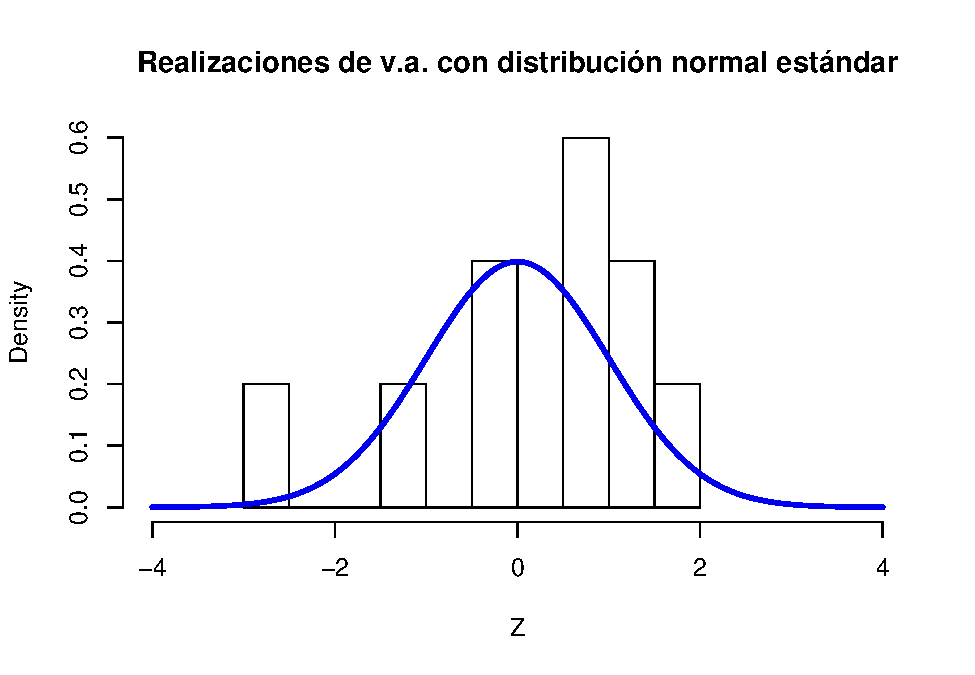
\includegraphics{NotaDeClaseLong_files/figure-latex/unnamed-chunk-8-1.pdf}

Ahora bien, una vez que tenemos estos valores, podemos tomar el cuadrado
de cada uno de ellos y sumarlos. De acuerdo con lo recién expuesto, esto
debería darnos una realizacion una variable aleatoria que se define de
esta forma. Esto sería una sola observación de una variable aleatoria
``suma de \(n\) variables aleatorias con distribución normal estándar''.

\begin{Shaded}
\begin{Highlighting}[]
\KeywordTok{print}\NormalTok{(Z)}
\end{Highlighting}
\end{Shaded}

\begin{verbatim}
##  [1]  0.56819281 -0.03564371  1.19478613 -2.61908879  0.56540354
##  [6]  0.72790979 -0.40139468  1.14647640 -1.23468688  1.80025080
\end{verbatim}

\begin{Shaded}
\begin{Highlighting}[]
\KeywordTok{print}\NormalTok{(Z}\OperatorTok{^}\DecValTok{2}\NormalTok{)}
\end{Highlighting}
\end{Shaded}

\begin{verbatim}
##  [1] 0.322843064 0.001270474 1.427513896 6.859626066 0.319681160
##  [6] 0.529852656 0.161117693 1.314408143 1.524451698 3.240902928
\end{verbatim}

\begin{Shaded}
\begin{Highlighting}[]
\KeywordTok{print}\NormalTok{(}\KeywordTok{sum}\NormalTok{(Z}\OperatorTok{^}\DecValTok{2}\NormalTok{))}
\end{Highlighting}
\end{Shaded}

\begin{verbatim}
## [1] 15.70167
\end{verbatim}

Podríamos repetir este proceso todas las veces que queramos, recolectar
los resultados que obtengamos y observar si las distintas realizaciones
siguen una distribución Ji-Cuadrado. Para simplicar el trabajo, se puede
usar una función que cree un vector en el que cada elemento contenga la
suma de los cuadrados de \(n\) realizaciones de variables aleatorias con
distribución normal estándar. La función SumZsq devuelve un vector con
\(m\) elementos, y en cada una de ellas hay una realización de la
variable aleatoria definida como \(\sum_{i=1}^n Z_i^2\).

\begin{Shaded}
\begin{Highlighting}[]
\NormalTok{ SumZsq <-}\StringTok{ }\ControlFlowTok{function}\NormalTok{(n, m)\{}
  \CommentTok{# n es la cantidad de N(0,1) que sumo}
  \CommentTok{# m es el numero de repeticiones que quiero}
\NormalTok{  v <-}\StringTok{ }\KeywordTok{vector}\NormalTok{()}
  \ControlFlowTok{for}\NormalTok{(i }\ControlFlowTok{in} \DecValTok{1}\OperatorTok{:}\NormalTok{m) \{}
\NormalTok{    z <-}\StringTok{ }\KeywordTok{rnorm}\NormalTok{(n, }\DecValTok{0}\NormalTok{, }\DecValTok{1}\NormalTok{)}
\NormalTok{    v[i] <-}\StringTok{ }\KeywordTok{sum}\NormalTok{(z}\OperatorTok{^}\DecValTok{2}\NormalTok{)}
\NormalTok{  \}}
  \KeywordTok{return}\NormalTok{(v)}
\NormalTok{ \}}
\end{Highlighting}
\end{Shaded}

De acuerdo con lo que dice la teoría estadística, esta variable se
distribuye Ji-Cuadrado con \(n\) grados de libertad ¿cómo podemos ver si
esto se cumple? En primer lugar, vamos a utilizar la función que recién
creamos para generar un vector que tenga \(m\) realizaciones de \(J\), y
luego vamos graficar el histograma de los valores de \(J\), junto con
una distribución Ji-Cuadrado con \(n\) grados de libertad, y luego
compararlos.

\begin{Shaded}
\begin{Highlighting}[]
\KeywordTok{SumZsq}\NormalTok{(}\DataTypeTok{n=}\DecValTok{10}\NormalTok{, }\DataTypeTok{m=}\DecValTok{40}\NormalTok{)}
\end{Highlighting}
\end{Shaded}

\begin{verbatim}
##  [1] 15.015513 14.526763  4.979442 16.211373  9.940637 17.793723  6.670770
##  [8]  4.816104  7.489471  3.952622  5.361086  4.299929  3.991255  9.590502
## [15]  9.860864 17.042254 12.572875 12.939149 10.432114  7.437532  7.235573
## [22]  6.962744  8.433115  3.148007 15.432692 10.395595  9.406276  5.609586
## [29] 12.185731  9.834225 10.611742  9.431430  7.955094  4.597255  8.615015
## [36]  6.740848 17.981920 10.995885 11.967719  9.488362
\end{verbatim}

\begin{Shaded}
\begin{Highlighting}[]
\NormalTok{n <-}\StringTok{ }\DecValTok{10} 
\NormalTok{m <-}\StringTok{ }\DecValTok{100}
\KeywordTok{hist}\NormalTok{(}\KeywordTok{SumZsq}\NormalTok{(n, m), }\DataTypeTok{freq =} \OtherTok{FALSE}\NormalTok{, }\DataTypeTok{breaks=}\DecValTok{30}\NormalTok{,}
     \DataTypeTok{main =} \StringTok{"Suma de cuadrado de realizaciones de N(0,1) }\CharTok{\textbackslash{}n}\StringTok{ y distribución Ji-Cuadrado"}\NormalTok{,}
     \DataTypeTok{xlim =} \KeywordTok{c}\NormalTok{(}\DecValTok{0}\NormalTok{,}\DecValTok{40}\NormalTok{), }\DataTypeTok{ylim =} \KeywordTok{c}\NormalTok{(}\DecValTok{0}\NormalTok{,.}\DecValTok{15}\NormalTok{))}
\KeywordTok{curve}\NormalTok{(}\KeywordTok{dchisq}\NormalTok{(x, }\DataTypeTok{df=}\NormalTok{n),}
      \DataTypeTok{from =} \DecValTok{0}\NormalTok{, }\DataTypeTok{to =} \DecValTok{40}\NormalTok{,}
      \DataTypeTok{col  =} \StringTok{"blue2"}\NormalTok{,}
      \DataTypeTok{lwd  =} \DecValTok{2}\NormalTok{,}
      \DataTypeTok{add  =} \OtherTok{TRUE}\NormalTok{)}
\KeywordTok{legend}\NormalTok{(}\StringTok{'topright'}\NormalTok{,}\DataTypeTok{legend =}  \KeywordTok{bquote}\NormalTok{(}\KeywordTok{atop}\NormalTok{(}\KeywordTok{paste}\NormalTok{(}\StringTok{"gl="}\NormalTok{,.(n)), }\KeywordTok{paste}\NormalTok{(}\StringTok{"reps="}\NormalTok{,.(m)))))}
\end{Highlighting}
\end{Shaded}

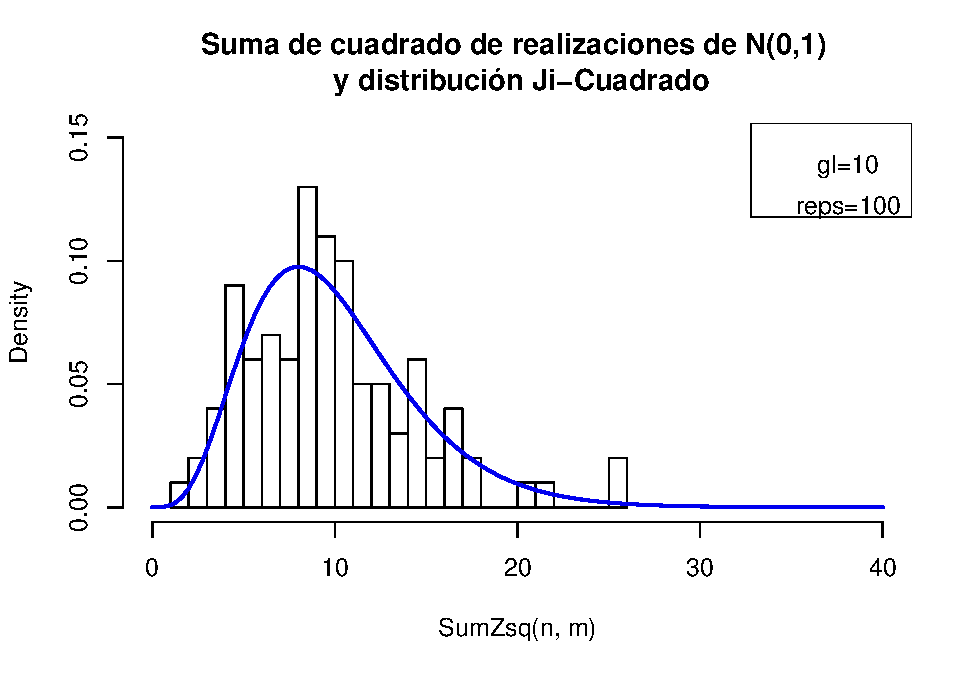
\includegraphics{NotaDeClaseLong_files/figure-latex/unnamed-chunk-11-1.pdf}

Probando distintas valores de \(m\), es decir, cantidad de repeticiones
(con \(n\) fijo en \(10\))

\begin{Shaded}
\begin{Highlighting}[]
\KeywordTok{par}\NormalTok{(}\DataTypeTok{mfrow=}\KeywordTok{c}\NormalTok{(}\DecValTok{2}\NormalTok{,}\DecValTok{2}\NormalTok{))}
\ControlFlowTok{for}\NormalTok{ (m }\ControlFlowTok{in} \KeywordTok{c}\NormalTok{(}\DecValTok{30}\NormalTok{, }\DecValTok{80}\NormalTok{, }\DecValTok{150}\NormalTok{, }\DecValTok{275}\NormalTok{, }\DecValTok{500}\NormalTok{))\{}
  \KeywordTok{set.seed}\NormalTok{(}\DecValTok{10}\NormalTok{)}
\NormalTok{  n <-}\StringTok{ }\DecValTok{10}
  \KeywordTok{hist}\NormalTok{(}\KeywordTok{SumZsq}\NormalTok{(n, m), }\DataTypeTok{freq =} \OtherTok{FALSE}\NormalTok{, }\DataTypeTok{breaks=}\DecValTok{20}\NormalTok{,}
       \DataTypeTok{xlim =} \KeywordTok{c}\NormalTok{(}\DecValTok{0}\NormalTok{,}\DecValTok{50}\NormalTok{), }\DataTypeTok{ylim =} \KeywordTok{c}\NormalTok{(}\DecValTok{0}\NormalTok{,.}\DecValTok{15}\NormalTok{))}
  \KeywordTok{curve}\NormalTok{(}\KeywordTok{dchisq}\NormalTok{(x, }\DataTypeTok{df=}\NormalTok{n),}
        \DataTypeTok{from =} \DecValTok{0}\NormalTok{, }\DataTypeTok{to =} \DecValTok{50}\NormalTok{,}
        \DataTypeTok{col  =} \StringTok{"blue2"}\NormalTok{,}
        \DataTypeTok{lwd  =} \DecValTok{2}\NormalTok{,}
        \DataTypeTok{add  =} \OtherTok{TRUE}\NormalTok{) }
  \KeywordTok{legend}\NormalTok{(}\StringTok{'topright'}\NormalTok{,}\DataTypeTok{legend =}  \KeywordTok{bquote}\NormalTok{(}\KeywordTok{atop}\NormalTok{(}\KeywordTok{paste}\NormalTok{(}\StringTok{"gl="}\NormalTok{,.(n)), }\KeywordTok{paste}\NormalTok{(}\StringTok{"reps="}\NormalTok{,.(m)))))}
\NormalTok{\}}
\end{Highlighting}
\end{Shaded}

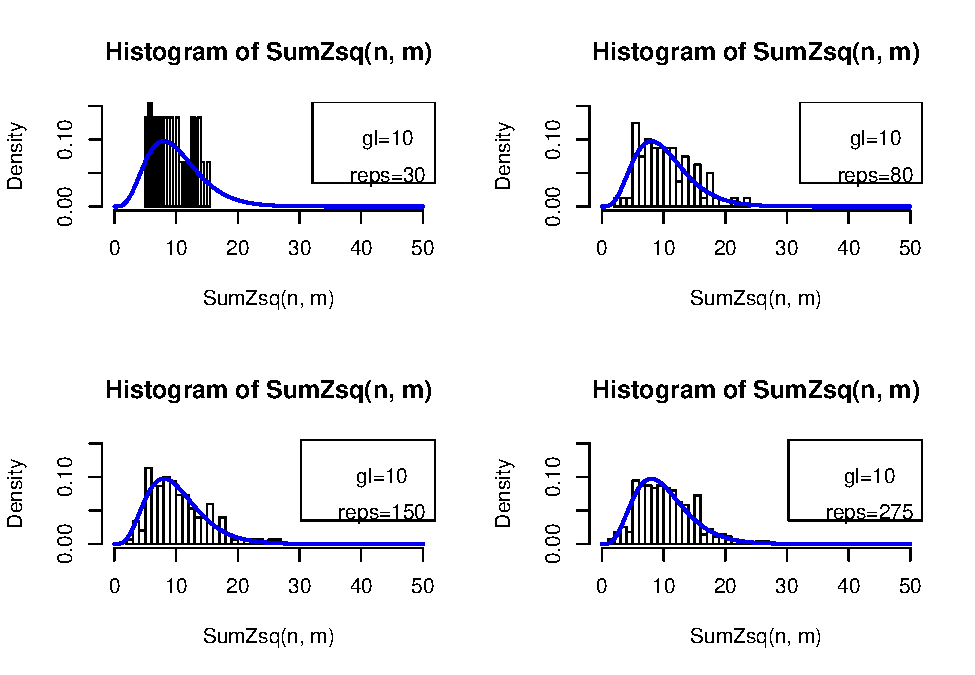
\includegraphics{NotaDeClaseLong_files/figure-latex/unnamed-chunk-12-1.pdf}
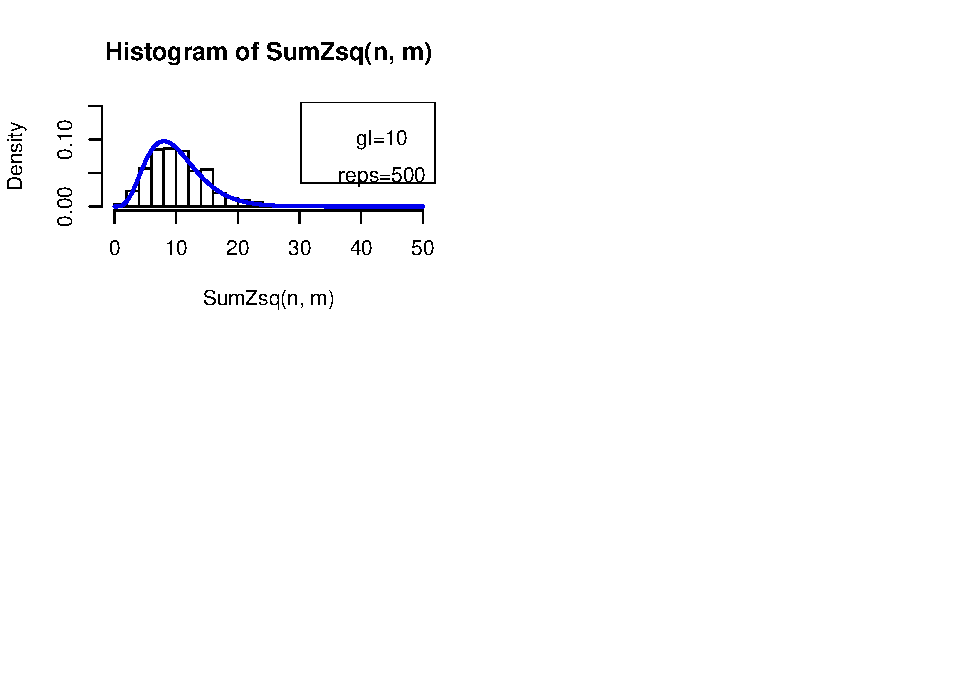
\includegraphics{NotaDeClaseLong_files/figure-latex/unnamed-chunk-12-2.pdf}

Probando con distintos valores de \(n\), es decir, cantidad de normales
estándar que estamos sumando (con \(m\) fijo en \(250\))

\begin{Shaded}
\begin{Highlighting}[]
\KeywordTok{par}\NormalTok{(}\DataTypeTok{mfrow=}\KeywordTok{c}\NormalTok{(}\DecValTok{2}\NormalTok{,}\DecValTok{2}\NormalTok{))}
\ControlFlowTok{for}\NormalTok{ (n }\ControlFlowTok{in} \KeywordTok{c}\NormalTok{(}\DecValTok{5}\NormalTok{, }\DecValTok{10}\NormalTok{, }\DecValTok{25}\NormalTok{, }\DecValTok{50}\NormalTok{))\{}
  \KeywordTok{set.seed}\NormalTok{(}\DecValTok{10}\NormalTok{)}
\NormalTok{  m <-}\StringTok{ }\DecValTok{250}
  \KeywordTok{hist}\NormalTok{(}\KeywordTok{SumZsq}\NormalTok{(n, m), }\DataTypeTok{freq =} \OtherTok{FALSE}\NormalTok{, }\DataTypeTok{breaks=}\DecValTok{20}\NormalTok{,}
       \DataTypeTok{main =} \KeywordTok{bquote}\NormalTok{(}\KeywordTok{paste}\NormalTok{(}\StringTok{"gl="}\NormalTok{,.(n), }\StringTok{", reps="}\NormalTok{,.(m))),}
       \DataTypeTok{xlim =} \KeywordTok{c}\NormalTok{(}\DecValTok{0}\NormalTok{,}\DecValTok{80}\NormalTok{), }\DataTypeTok{ylim =} \KeywordTok{c}\NormalTok{(}\DecValTok{0}\NormalTok{,.}\DecValTok{15}\NormalTok{))}
  \KeywordTok{curve}\NormalTok{(}\KeywordTok{dchisq}\NormalTok{(x, }\DataTypeTok{df=}\NormalTok{n),}
        \DataTypeTok{from =} \DecValTok{0}\NormalTok{, }\DataTypeTok{to =} \DecValTok{80}\NormalTok{,}
        \DataTypeTok{col  =} \StringTok{"blue2"}\NormalTok{,}
        \DataTypeTok{lwd  =} \DecValTok{2}\NormalTok{,}
        \DataTypeTok{add  =} \OtherTok{TRUE}\NormalTok{) }
\NormalTok{\}}
\end{Highlighting}
\end{Shaded}

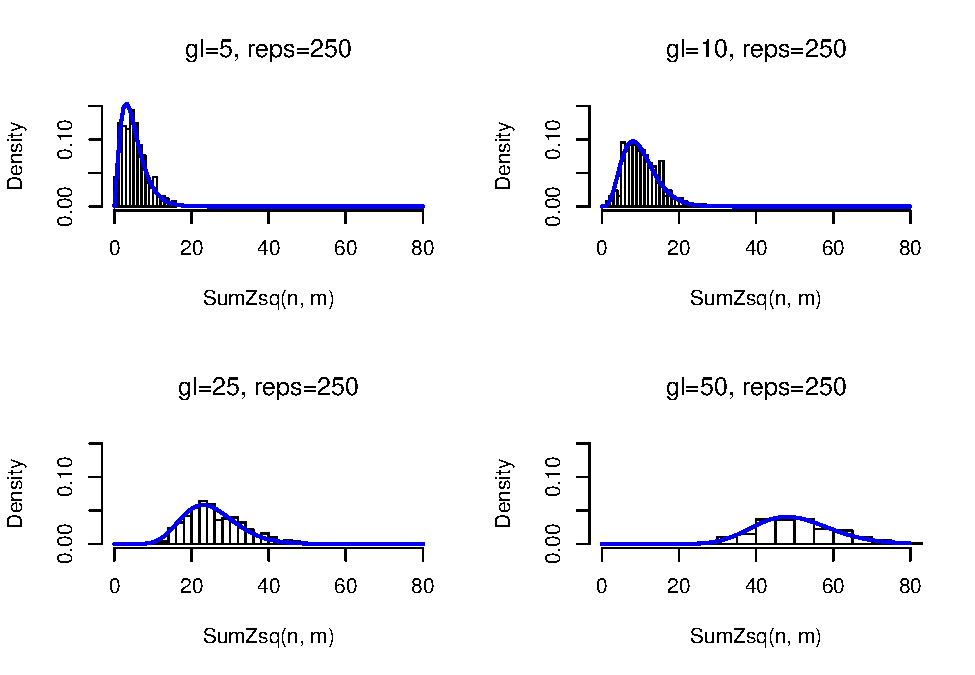
\includegraphics{NotaDeClaseLong_files/figure-latex/unnamed-chunk-13-1.pdf}

Haciendo simulaciones, parece cumplirse que la suma de los cuadrados
variables aleatorias normales estándar se distribuya sea una variable
aleatoria que se distribuye Ji-Cuadrado con \(n\) grados de libertad.

\hypertarget{distribucion-t-de-student}{%
\subsubsection{Distribución t de
Student}\label{distribucion-t-de-student}}

Siendo \(Z \sim N(0,\,1)\) y \(J \sim \chi^2_n\), una variable aleatoria
con distribución \(t\) de Student se define como el cociente entre una
variable aleatoria normal estándar y la raíz cuadrada de una variable
aleatoria Ji-Cuadrado sobre sus grados de libertad

\[T = \frac{Z}{\sqrt{J/n}},\] Las funciones de densidad, probabilidad
acumulada, cuantiles y generación de números aleatorios en R son las
siguientes:

\begin{Shaded}
\begin{Highlighting}[]
\CommentTok{#df = degrees of freedom = grados de libertad}
\CommentTok{#dt(x, df, ncp, log = FALSE)}
\CommentTok{#pt(q, df, ncp, lower.tail = TRUE, log.p = FALSE)}
\CommentTok{#qt(p, df, ncp, lower.tail = TRUE, log.p = FALSE)}
\CommentTok{#rt(n, df, ncp)}
\end{Highlighting}
\end{Shaded}

Se puede mostrar a través de simulaciones que se cumple la relación
entre la distribución \(t\) y las distribuciones normal estándar y
Ji-Cuadrado. Para esto, vamos a seguir el mismo procedimiento realizado
anteriormente, aunque con menos ``detalle'' y una mejor forma de
implementarlo en R.

\begin{Shaded}
\begin{Highlighting}[]
\KeywordTok{set.seed}\NormalTok{(}\DecValTok{285}\NormalTok{)}

\NormalTok{draw.T <-}\StringTok{ }\ControlFlowTok{function}\NormalTok{(n)\{}
  \CommentTok{# n es grados de libertad}
\NormalTok{  Z <-}\StringTok{ }\KeywordTok{rnorm}\NormalTok{(}\DecValTok{1}\NormalTok{, }\DecValTok{0}\NormalTok{, }\DecValTok{1}\NormalTok{)}
\NormalTok{  J <-}\StringTok{ }\KeywordTok{rchisq}\NormalTok{(}\DecValTok{1}\NormalTok{, n)}
\NormalTok{  T <-}\StringTok{ }\NormalTok{Z }\OperatorTok{/}\StringTok{ }\KeywordTok{sqrt}\NormalTok{(J}\OperatorTok{/}\NormalTok{n)}
  \KeywordTok{return}\NormalTok{(T)}
\NormalTok{\}}

\KeywordTok{draw.T}\NormalTok{(}\DecValTok{5}\NormalTok{);}\KeywordTok{draw.T}\NormalTok{(}\DecValTok{5}\NormalTok{);}\KeywordTok{draw.T}\NormalTok{(}\DecValTok{5}\NormalTok{);}\KeywordTok{draw.T}\NormalTok{(}\DecValTok{5}\NormalTok{);}\KeywordTok{draw.T}\NormalTok{(}\DecValTok{5}\NormalTok{);}\KeywordTok{draw.T}\NormalTok{(}\DecValTok{5}\NormalTok{);}\KeywordTok{draw.T}\NormalTok{(}\DecValTok{5}\NormalTok{)}
\end{Highlighting}
\end{Shaded}

\begin{verbatim}
## [1] 0.6433665
\end{verbatim}

\begin{verbatim}
## [1] 0.8512115
\end{verbatim}

\begin{verbatim}
## [1] 0.9484228
\end{verbatim}

\begin{verbatim}
## [1] -0.4790173
\end{verbatim}

\begin{verbatim}
## [1] -0.6630038
\end{verbatim}

\begin{verbatim}
## [1] 0.4028808
\end{verbatim}

\begin{verbatim}
## [1] -1.429738
\end{verbatim}

\begin{Shaded}
\begin{Highlighting}[]
\NormalTok{vec.T <-}\StringTok{ }\ControlFlowTok{function}\NormalTok{(n, m)\{}
  \CommentTok{# n: grados de libertad}
  \CommentTok{# m: el numero de repeticiones que quiero}
\NormalTok{  v <-}\StringTok{ }\KeywordTok{vector}\NormalTok{()}
  \ControlFlowTok{for}\NormalTok{(i }\ControlFlowTok{in} \DecValTok{1}\OperatorTok{:}\NormalTok{m)\{}
\NormalTok{    v[i] <-}\StringTok{ }\KeywordTok{draw.T}\NormalTok{(n)}
\NormalTok{  \}}
  \KeywordTok{return}\NormalTok{(v)}
\NormalTok{\}}

\NormalTok{n <-}\StringTok{ }\DecValTok{10} 
\NormalTok{m <-}\StringTok{ }\DecValTok{100}



\KeywordTok{hist}\NormalTok{(}\KeywordTok{vec.T}\NormalTok{(n, m), }\DataTypeTok{freq =} \OtherTok{FALSE}\NormalTok{, }\DataTypeTok{breaks=}\DecValTok{30}\NormalTok{,}
     \DataTypeTok{main =} \StringTok{"Suma de cuadrados de realizaciones de N(0,1) }\CharTok{\textbackslash{}n}\StringTok{ y distribución Ji-Cuadrado"}\NormalTok{,}
     \DataTypeTok{xlim =} \KeywordTok{c}\NormalTok{(}\OperatorTok{-}\DecValTok{10}\NormalTok{,}\DecValTok{10}\NormalTok{), }\DataTypeTok{ylim =} \KeywordTok{c}\NormalTok{(}\DecValTok{0}\NormalTok{,.}\DecValTok{5}\NormalTok{))}
\KeywordTok{curve}\NormalTok{(}\KeywordTok{dchisq}\NormalTok{(x, }\DataTypeTok{df=}\NormalTok{n),}
      \DataTypeTok{from =} \DecValTok{-10}\NormalTok{, }\DataTypeTok{to =} \DecValTok{10}\NormalTok{,}
      \DataTypeTok{col  =} \StringTok{"blue2"}\NormalTok{,}
      \DataTypeTok{lwd  =} \DecValTok{2}\NormalTok{,}
      \DataTypeTok{add  =} \OtherTok{TRUE}\NormalTok{)}
\KeywordTok{legend}\NormalTok{(}\StringTok{'topright'}\NormalTok{,}\DataTypeTok{legend =}  \KeywordTok{bquote}\NormalTok{(}\KeywordTok{atop}\NormalTok{(}\KeywordTok{paste}\NormalTok{(}\StringTok{"gl="}\NormalTok{,.(n)), }\KeywordTok{paste}\NormalTok{(}\StringTok{"reps="}\NormalTok{,.(m)))))}
\end{Highlighting}
\end{Shaded}

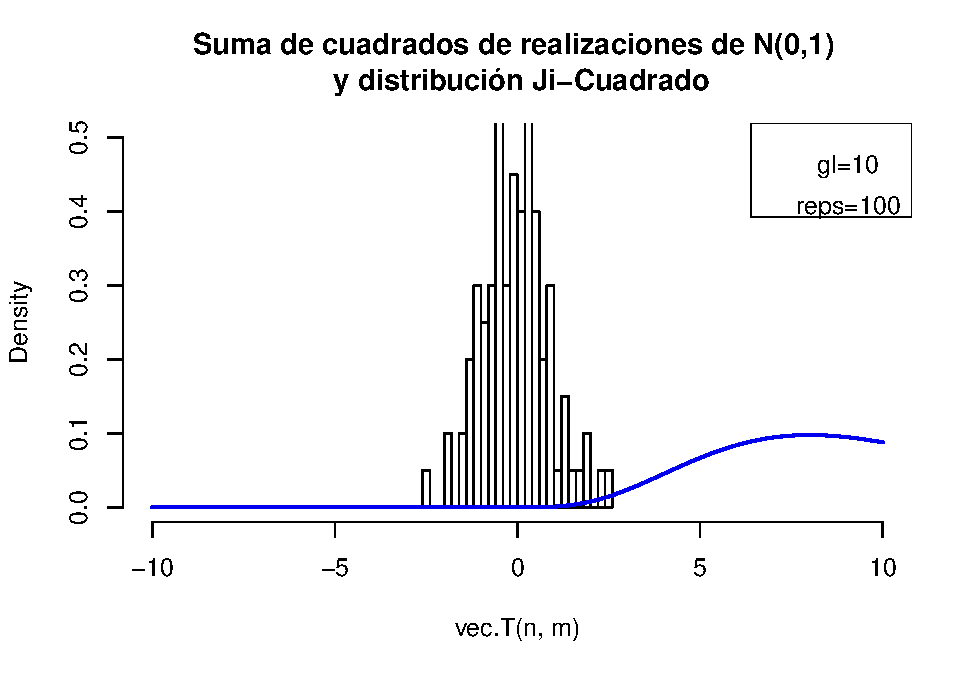
\includegraphics{NotaDeClaseLong_files/figure-latex/unnamed-chunk-15-1.pdf}

\begin{Shaded}
\begin{Highlighting}[]
\NormalTok{Plot1Simul.T <-}\StringTok{ }\ControlFlowTok{function}\NormalTok{(n,m)\{}
  \KeywordTok{hist}\NormalTok{(}\KeywordTok{vec.T}\NormalTok{(n, m), }\DataTypeTok{freq =} \OtherTok{FALSE}\NormalTok{, }\DataTypeTok{breaks=}\DecValTok{30}\NormalTok{,}
       \DataTypeTok{main =} \KeywordTok{bquote}\NormalTok{(}\KeywordTok{paste}\NormalTok{(}\StringTok{"gl="}\NormalTok{,.(n), }\StringTok{", reps="}\NormalTok{,.(m))),}
       \DataTypeTok{xlab =} \StringTok{""}\NormalTok{,}
       \DataTypeTok{xlim =} \KeywordTok{c}\NormalTok{(}\OperatorTok{-}\DecValTok{10}\NormalTok{,}\DecValTok{10}\NormalTok{), }\DataTypeTok{ylim =} \KeywordTok{c}\NormalTok{(}\DecValTok{0}\NormalTok{,.}\DecValTok{5}\NormalTok{))}
  \KeywordTok{curve}\NormalTok{(}\KeywordTok{dt}\NormalTok{(x, }\DataTypeTok{df=}\NormalTok{n),}
        \DataTypeTok{from =} \DecValTok{-10}\NormalTok{, }\DataTypeTok{to =} \DecValTok{10}\NormalTok{,}
        \DataTypeTok{col  =} \StringTok{"blue2"}\NormalTok{,}
        \DataTypeTok{lwd  =} \DecValTok{2}\NormalTok{,}
        \DataTypeTok{add  =} \OtherTok{TRUE}\NormalTok{)}
\NormalTok{\}}


\KeywordTok{Plot1Simul.T}\NormalTok{(}\DataTypeTok{n=}\DecValTok{100}\NormalTok{,}\DataTypeTok{m=}\DecValTok{1000}\NormalTok{)}
\end{Highlighting}
\end{Shaded}

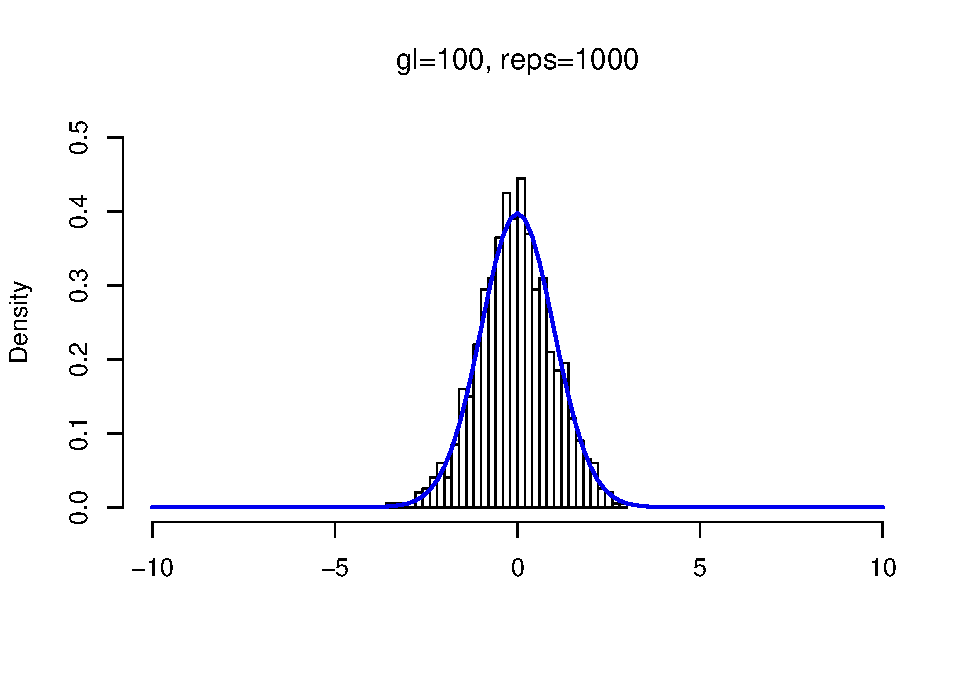
\includegraphics{NotaDeClaseLong_files/figure-latex/unnamed-chunk-15-2.pdf}

\begin{Shaded}
\begin{Highlighting}[]
\CommentTok{# cambiando el número de repeticiones}

\NormalTok{PlotSimulReps.T <-}\StringTok{ }\ControlFlowTok{function}\NormalTok{(n, m.opt, p.rows, p.cols)\{}
  \CommentTok{# n: grados de libertad }
  \CommentTok{# m.opt: vector de numero de distintas repeticiones}
  \CommentTok{# p.row: numero de filas en el plot dividido}
  \CommentTok{# p.col: numero de columnas en el plot dividido}
  \CommentTok{# restriccion: length(m.opt) = p.row * p.col}
  \ControlFlowTok{if}\NormalTok{(}\KeywordTok{length}\NormalTok{(m.opt)}\OperatorTok{<}\DecValTok{9}\NormalTok{)\{p.cols.def<-}\DecValTok{2}\NormalTok{\} }\ControlFlowTok{else}\NormalTok{ \{p.cols.def<-}\DecValTok{3}\NormalTok{\}}
  \ControlFlowTok{if}\NormalTok{(}\KeywordTok{missing}\NormalTok{(p.rows) }\OperatorTok{|}\StringTok{ }\KeywordTok{missing}\NormalTok{(p.cols))\{}
\NormalTok{    p.cols =}\StringTok{ }\NormalTok{p.cols.def}
\NormalTok{    p.rows =}\StringTok{ }\KeywordTok{ceiling}\NormalTok{(}\KeywordTok{length}\NormalTok{(m.opt)}\OperatorTok{/}\NormalTok{p.cols.def)\}}
  \KeywordTok{par}\NormalTok{(}\DataTypeTok{mfrow=}\KeywordTok{c}\NormalTok{(p.rows,p.cols), }\DataTypeTok{mar=}\KeywordTok{c}\NormalTok{(}\DecValTok{2}\NormalTok{,}\DecValTok{2}\NormalTok{,}\DecValTok{2}\NormalTok{,}\DecValTok{2}\NormalTok{))}
  \ControlFlowTok{if}\NormalTok{(}\KeywordTok{missing}\NormalTok{(p.rows) }\OperatorTok{|}\StringTok{ }\KeywordTok{missing}\NormalTok{(p.cols))\{}
\NormalTok{   p.cols =}\StringTok{ }\DecValTok{2}
\NormalTok{   p.rows =}\StringTok{ }\KeywordTok{ceiling}\NormalTok{(}\KeywordTok{length}\NormalTok{(m.opt)}\OperatorTok{/}\DecValTok{2}\NormalTok{)\}}
  \KeywordTok{par}\NormalTok{(}\DataTypeTok{mfrow=}\KeywordTok{c}\NormalTok{(p.rows,p.cols))}
  \ControlFlowTok{for}\NormalTok{ (m }\ControlFlowTok{in}\NormalTok{ m.opt)\{}
    \KeywordTok{Plot1Simul.T}\NormalTok{(n,m)}
\NormalTok{  \}}
\NormalTok{\}}

\KeywordTok{PlotSimulReps.T}\NormalTok{(}\DataTypeTok{n=}\DecValTok{8}\NormalTok{, }\DataTypeTok{m.opt =} \KeywordTok{c}\NormalTok{(}\DecValTok{20}\NormalTok{,}\DecValTok{50}\NormalTok{,}\DecValTok{100}\NormalTok{,}\DecValTok{500}\NormalTok{,}\DecValTok{1000}\NormalTok{))}
  
\CommentTok{# cambiando los grados de libertad}

\NormalTok{PlotSimulDF.T <-}\StringTok{ }\ControlFlowTok{function}\NormalTok{(m, n.opt, p.rows, p.cols)\{}
  \CommentTok{# n: grados de libertad }
  \CommentTok{# m.opt: vector de numero de distintas repeticiones}
  \CommentTok{# p.row: numero de filas en el plot dividido}
  \CommentTok{# p.col: numero de columnas en el plot dividido}
  \CommentTok{# restriccion: length(m.opt) = p.row * p.col}
  \ControlFlowTok{if}\NormalTok{(}\KeywordTok{length}\NormalTok{(n.opt)}\OperatorTok{<}\DecValTok{9}\NormalTok{)\{p.cols.def<-}\DecValTok{2}\NormalTok{\} }\ControlFlowTok{else}\NormalTok{ \{p.cols.def<-}\DecValTok{3}\NormalTok{\}}
  \ControlFlowTok{if}\NormalTok{(}\KeywordTok{missing}\NormalTok{(p.rows) }\OperatorTok{|}\StringTok{ }\KeywordTok{missing}\NormalTok{(p.cols))\{}
\NormalTok{    p.cols <-}\StringTok{ }\NormalTok{p.cols.def}
\NormalTok{    p.rows <-}\StringTok{ }\KeywordTok{ceiling}\NormalTok{(}\KeywordTok{length}\NormalTok{(n.opt)}\OperatorTok{/}\NormalTok{p.cols.def)\}}
  \KeywordTok{par}\NormalTok{(}\DataTypeTok{mfrow =} \KeywordTok{c}\NormalTok{(p.rows,p.cols), }\DataTypeTok{mar =} \KeywordTok{c}\NormalTok{(}\DecValTok{2}\NormalTok{,}\DecValTok{2}\NormalTok{,}\DecValTok{2}\NormalTok{,}\DecValTok{2}\NormalTok{))}
  \ControlFlowTok{for}\NormalTok{ (n }\ControlFlowTok{in}\NormalTok{ n.opt)\{}
    \KeywordTok{Plot1Simul.T}\NormalTok{(n,m)}
\NormalTok{  \}}
\NormalTok{\}}

\KeywordTok{PlotSimulDF.T}\NormalTok{(}\DataTypeTok{m=}\DecValTok{200}\NormalTok{, }\DataTypeTok{n.opt =} \KeywordTok{c}\NormalTok{(}\DecValTok{1}\NormalTok{,}\DecValTok{2}\NormalTok{,}\DecValTok{3}\NormalTok{,}\DecValTok{4}\NormalTok{,}\DecValTok{5}\NormalTok{,}\DecValTok{6}\NormalTok{,}\DecValTok{8}\NormalTok{))}
\end{Highlighting}
\end{Shaded}

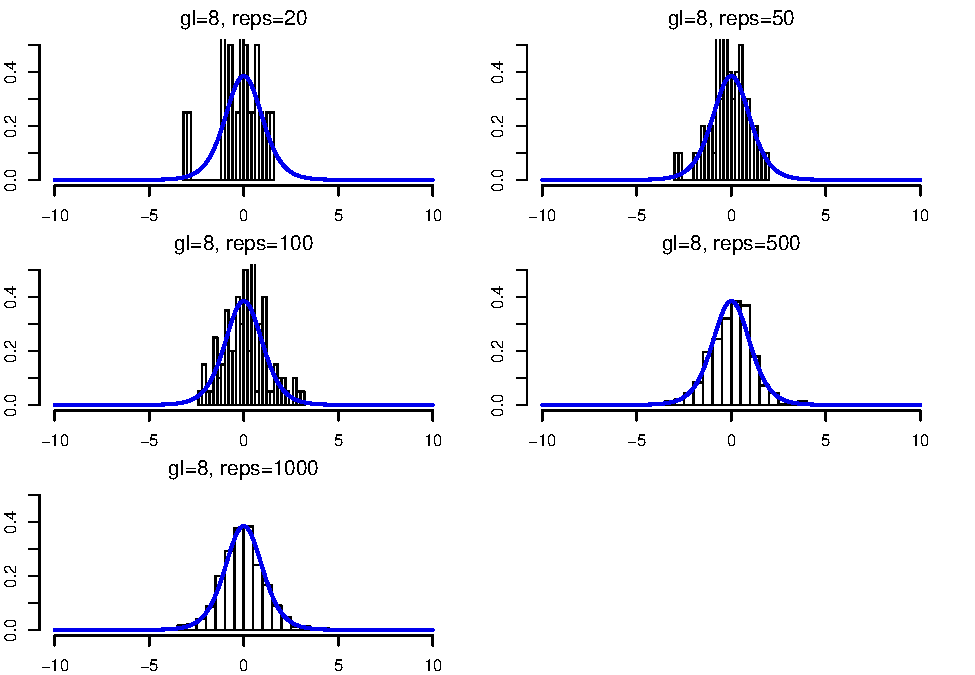
\includegraphics{NotaDeClaseLong_files/figure-latex/unnamed-chunk-15-3.pdf}

\begin{Shaded}
\begin{Highlighting}[]
\KeywordTok{PlotSimulDF.T}\NormalTok{(}\DataTypeTok{m=}\DecValTok{200}\NormalTok{, }\DataTypeTok{n.opt =} \KeywordTok{c}\NormalTok{(}\DecValTok{5}\NormalTok{,}\DecValTok{10}\NormalTok{,}\DecValTok{15}\NormalTok{,}\DecValTok{20}\NormalTok{))}
\end{Highlighting}
\end{Shaded}

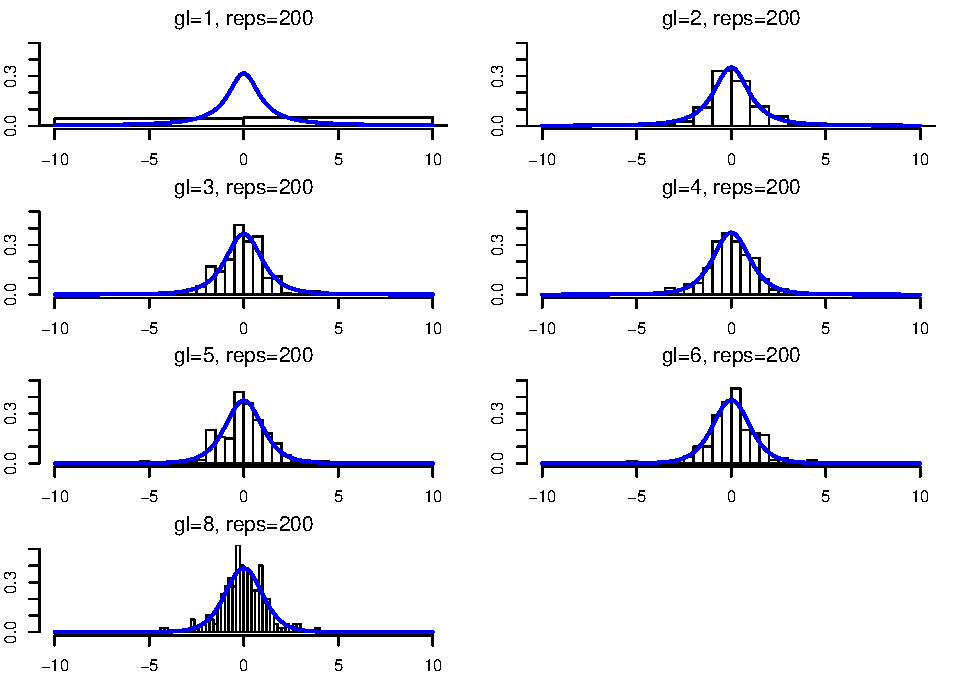
\includegraphics{NotaDeClaseLong_files/figure-latex/unnamed-chunk-15-4.pdf}
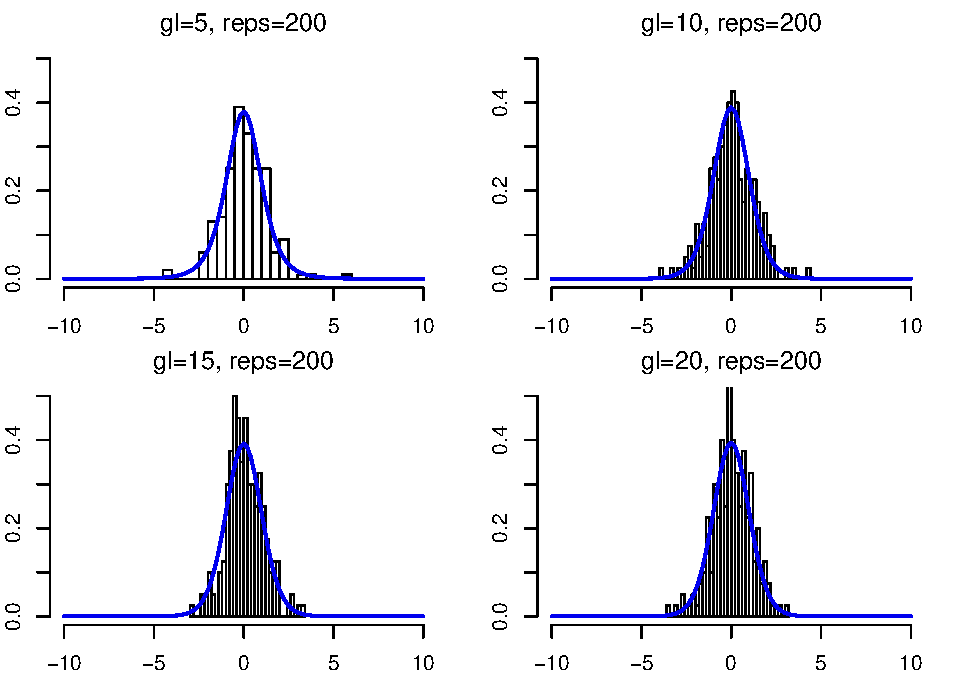
\includegraphics{NotaDeClaseLong_files/figure-latex/unnamed-chunk-15-5.pdf}

\hypertarget{distribucion-f-de-fisher-o-de-snedecor}{%
\subsubsection{Distribución F de Fisher o de
Snedecor}\label{distribucion-f-de-fisher-o-de-snedecor}}

Siendo \(J_1 \sim \chi^2(n_1)\) y \(J_2 \sim \chi^2(n_2)\) dos
distribuciones Ji-Cuadrado con respectivamente \(n_1\) y \(n_2\) grados
de libertad, se define la distribución F como el cociente de dos
distribuciones Ji-Cuadrado escaladas por sus grados de libertad.

\[F = \frac{J_1 / n_1}{J_2 / n_2},\] Las funciones en R para la función
de densidad, función de probabilidad acumulada, función de cuantiles y
generación de números aleatorios son:

\begin{Shaded}
\begin{Highlighting}[]
\CommentTok{#df = degrees of freedom = grados de libertad}
\CommentTok{#dt(x, df_num, df_denom, ncp, log = FALSE)}
\CommentTok{#pt(q, df_num, df_denom, ncp, lower.tail = TRUE, log.p = FALSE)}
\CommentTok{#qt(p, df_num, df_denom, ncp, lower.tail = TRUE, log.p = FALSE)}
\CommentTok{#rt(n, df_num, df_denom, ncp)}
\end{Highlighting}
\end{Shaded}

A través de simulaciones, se puede verificar que una distribución F se
define de esta forma

\hypertarget{momentos}{%
\section{Momentos}\label{momentos}}

\hypertarget{propiedades-de-fgm}{%
\subsection{Propiedades de FGM:}\label{propiedades-de-fgm}}

Sean \(X,\;Y\) dos variables aleatorias independientes, y \(a,\;b\) dos
números reales.

\begin{itemize}
\item
  \(\varphi_{aX} (t) = \varphi_X (at)\)
\item
  \(\varphi_{X+Y} (t) = \varphi_X (t) \cdot \varphi_X (t)\)
\item
  \(\varphi_{aX+b} (t) = e^{bt} \varphi_{aX} (t)\)
\end{itemize}

Pensar qué se puede hacer con simulaciones

\hypertarget{fgm-de-distintas-distribuciones}{%
\subsection{FGM de distintas
distribuciones}\label{fgm-de-distintas-distribuciones}}

Distribución Binomial, o Bernoulli con \(m=1\)

\[
\varphi_x (t) = (pe^t + q)^m
\]

Distribución de Poisson \[
\varphi_x (t) = e^{- \lambda (1-e^t)} = e^{\lambda (e^t - 1 )}
\]

Distribución geométrica

\[
\varphi_x (t) = \frac{pe^t }{1-qe^t}
\]

Distribución normal estándar \[
\varphi_x (t) = e^{ \frac{1}{2} t^2}
\]

Distribución normal \[
\varphi_x (t) = e^{ \mu t + \frac{1}{2} \sigma^2 t^2}
\]

Distribución gamma

\[
\varphi_x (t) = (1 - \beta t)^{- \alpha}
\]

Casos especiales:

\begin{itemize}
\item
  Ji-Cuadrado \[
  \varphi_x (t) = (1 - 2 t)^{- n/2}
  \]
\item
  Exponencial \[
  \varphi_x (t) = (1 - \beta t)^{-1} = \frac{1}{1- \beta t}
  \]
\end{itemize}

\hypertarget{ley-de-los-grandes-numeros-y-teorema-central-del-limite}{%
\section{Ley de los Grandes Números y Teorema Central del
Límite}\label{ley-de-los-grandes-numeros-y-teorema-central-del-limite}}

\hypertarget{estimadores}{%
\section{Estimadores}\label{estimadores}}

\hypertarget{propiedades}{%
\subsection{Propiedades}\label{propiedades}}

\hypertarget{insesgamiento}{%
\subsubsection{Insesgamiento}\label{insesgamiento}}

Sesgo

Insesgamiento Asintótico

\hypertarget{consistencia}{%
\subsubsection{Consistencia}\label{consistencia}}

\hypertarget{eficiencia-relativa}{%
\subsubsection{Eficiencia relativa}\label{eficiencia-relativa}}

Varianza

Error cuadrático medio

\hypertarget{eficiencia-en-sentido-absoluto}{%
\subsubsection{Eficiencia en sentido
absoluto}\label{eficiencia-en-sentido-absoluto}}

Cota de Rao-Cramer

\hypertarget{metodos-de-estimacion}{%
\subsection{Métodos de Estimación}\label{metodos-de-estimacion}}

\hypertarget{metodo-de-momentos}{%
\subsubsection{Método de momentos}\label{metodo-de-momentos}}

\hypertarget{estimacion-de-maxima-verosimilitud}{%
\subsubsection{Estimación de Máxima
Verosimilitud}\label{estimacion-de-maxima-verosimilitud}}

Esto estoy segura que se hace. al menos en py

\hypertarget{intervalos-de-confianza}{%
\section{Intervalos de Confianza}\label{intervalos-de-confianza}}

\hypertarget{una-poblacion}{%
\subsection{Una población}\label{una-poblacion}}

Método de la cantidad pivotal

Media \(\mu\) de una variable aleatoria \(x\) con distribución normal
con \(\sigma\) conocido

Media \(\mu\) de una variable aleatoria \(x\) con distribución normal
con \(\sigma\) desconocido

Varianza \(\sigma^2\) de una variable aleatoria \(x\) con distribución
normal con \(\sigma\) desconocido

IC asintótico para proporción \(p\) de una varaible aleatoria con
distribucón Bernoulli

\hypertarget{dos-poblaciones}{%
\subsection{Dos poblaciones}\label{dos-poblaciones}}

IC para diferencia de medias \(\mu_1 - \mu_2\) de dos poblaciones
\(x,\; y\) con distribuciones normales independientes con desvíos
estándar \(\sigma_1\) y\(\sigma_2\) conocidos

IC para diferencia de medias \(\mu_1 - \mu_2\) de dos poblaciones
\(x,\; y\) con distribuciones normales independientes con desvíos
estándar \(\sigma_1\) y\(\sigma_2\) desconocidos pero supuestamente
iguales, \(\sigma_1 = \sigma_2 = \sigma\)

\hypertarget{test-de-hipotesis}{%
\section{Test de Hipótesis}\label{test-de-hipotesis}}

\hypertarget{regresion-lineal}{%
\section{Regresión Lineal}\label{regresion-lineal}}

\hypertarget{minimos-cuadrados-ordinarios}{%
\subsection{Mínimos Cuadrados
Ordinarios}\label{minimos-cuadrados-ordinarios}}

\hypertarget{inferencia-estadistica-en-modelos-de-regresion}{%
\subsection{Inferencia estadística en modelos de
regresión}\label{inferencia-estadistica-en-modelos-de-regresion}}

Acá basarme un poco en lo que tengo de Ezequiel, ver que puedo
condimentar con las cosas de Econometría (creo que poco)

Ver si puedo armar funciones que computen todo lo que hace MCO. Dejarlo
como ejercicio y al final ponerlo como solución

\hypertarget{anova}{%
\section{ANOVA}\label{anova}}

\hypertarget{bondad-de-ajuste-e-independencia-de-atributos}{%
\section{Bondad de Ajuste e Independencia de
Atributos}\label{bondad-de-ajuste-e-independencia-de-atributos}}

En la literatura de econ vi que usan estos tests para probar la
normalidad de distribuciones. Por ejemplo, Reinhart y Rogoff.

\hypertarget{test-ji-cuadrado}{%
\subsection{Test Ji-Cuadrado}\label{test-ji-cuadrado}}

Ajuste con distintas variables

\hypertarget{test-kolmogorov-smirnov}{%
\subsection{Test Kolmogorov-Smirnov}\label{test-kolmogorov-smirnov}}

ks.test

\hypertarget{otras-medidas-de-bondad-del-ajuste}{%
\subsection{Otras medidas de bondad del
ajuste}\label{otras-medidas-de-bondad-del-ajuste}}

\begin{Shaded}
\begin{Highlighting}[]
\NormalTok{x <-}\StringTok{ }\KeywordTok{seq}\NormalTok{(}\DecValTok{1}\OperatorTok{:}\DecValTok{50}\NormalTok{)}

\KeywordTok{curve}\NormalTok{( }\KeywordTok{dchisq}\NormalTok{(x, }\DataTypeTok{df=}\DecValTok{5}\NormalTok{), }\DataTypeTok{col=}\StringTok{'black'}\NormalTok{, }\DataTypeTok{lwd =} \DecValTok{2}\NormalTok{,}
       \DataTypeTok{from =} \DecValTok{0}\NormalTok{, }\DataTypeTok{to =} \DecValTok{50}\NormalTok{,}
       \DataTypeTok{ylab =} \StringTok{'p(x)'}\NormalTok{,}
       \DataTypeTok{main =} \StringTok{'Distribución Ji-Cuadrado'}\NormalTok{)}
\KeywordTok{curve}\NormalTok{( }\KeywordTok{dchisq}\NormalTok{(x, }\DataTypeTok{df=}\DecValTok{1}\NormalTok{), }\DataTypeTok{col=}\StringTok{'gray'}\NormalTok{, }\DataTypeTok{add=}\OtherTok{TRUE}\NormalTok{)}
\KeywordTok{curve}\NormalTok{( }\KeywordTok{dchisq}\NormalTok{(x, }\DataTypeTok{df=}\DecValTok{10}\NormalTok{), }\DataTypeTok{col=}\StringTok{'black'}\NormalTok{, }\DataTypeTok{add=}\OtherTok{TRUE}\NormalTok{, }\DataTypeTok{lty =} \DecValTok{2}\NormalTok{)}
\KeywordTok{curve}\NormalTok{( }\KeywordTok{dchisq}\NormalTok{(x, }\DataTypeTok{df=}\DecValTok{20}\NormalTok{), }\DataTypeTok{col=}\StringTok{'black'}\NormalTok{, }\DataTypeTok{add=}\OtherTok{TRUE}\NormalTok{, }\DataTypeTok{lty =} \DecValTok{3}\NormalTok{ )}

\KeywordTok{legend}\NormalTok{(}\StringTok{'topright'}\NormalTok{, }
      \KeywordTok{expression}\NormalTok{(gl}\OperatorTok{==}\DecValTok{1}\NormalTok{, gl}\OperatorTok{==}\DecValTok{5}\NormalTok{, gl}\OperatorTok{==}\DecValTok{10}\NormalTok{, gl}\OperatorTok{==}\DecValTok{20}\NormalTok{),}
      \DataTypeTok{lwd =} \KeywordTok{c}\NormalTok{(}\DecValTok{1}\NormalTok{, }\DecValTok{2}\NormalTok{, }\DecValTok{1}\NormalTok{, }\DecValTok{1}\NormalTok{),}
      \DataTypeTok{lty =} \KeywordTok{c}\NormalTok{(}\DecValTok{1}\NormalTok{,}\DecValTok{1}\NormalTok{, }\DecValTok{2}\NormalTok{, }\DecValTok{3}\NormalTok{),}
      \DataTypeTok{col =} \KeywordTok{c}\NormalTok{(}\StringTok{'grey'}\NormalTok{,}\StringTok{'black'}\NormalTok{, }\StringTok{'black'}\NormalTok{, }\StringTok{'black'}\NormalTok{))}
\end{Highlighting}
\end{Shaded}

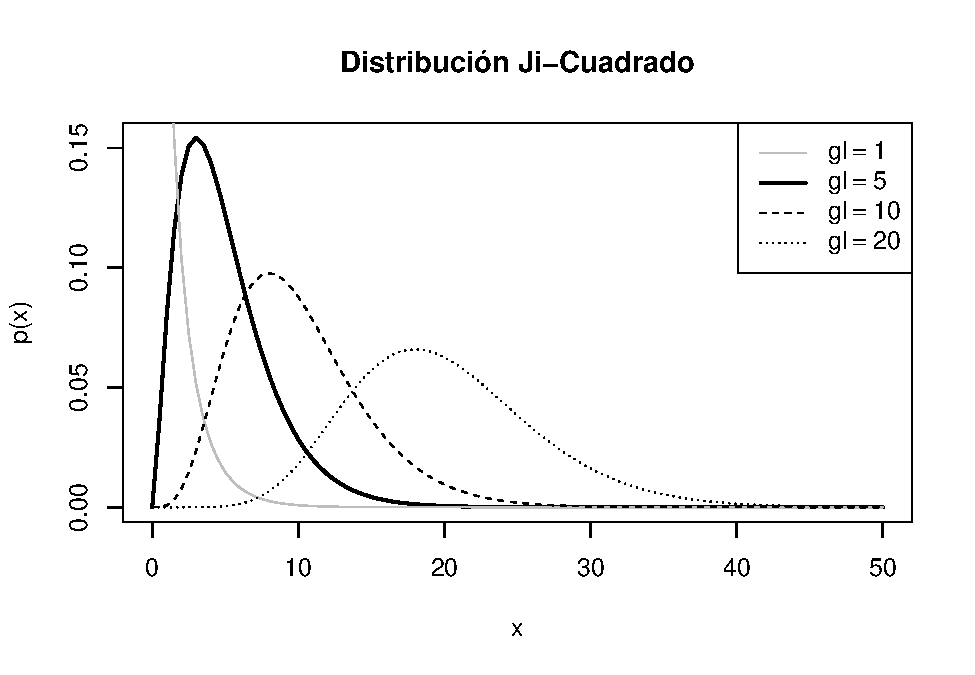
\includegraphics{NotaDeClaseLong_files/figure-latex/unnamed-chunk-18-1.pdf}

\begin{Shaded}
\begin{Highlighting}[]
\CommentTok{# Armar tabla}
\CommentTok{# Data wrangling para calcular el estadístico}
\CommentTok{# Test}

\KeywordTok{curve}\NormalTok{( }\KeywordTok{dchisq}\NormalTok{(x, }\DataTypeTok{df=}\DecValTok{5}\NormalTok{), }\DataTypeTok{col=}\StringTok{'black'}\NormalTok{, }\DataTypeTok{lwd =} \DecValTok{2}\NormalTok{,}
       \DataTypeTok{from =} \DecValTok{0}\NormalTok{, }\DataTypeTok{to =} \DecValTok{20}\NormalTok{,}
       \DataTypeTok{ylab =} \StringTok{'p(x)'}\NormalTok{,}
       \DataTypeTok{main =} \StringTok{'Distribución Ji-Cuadrado'}\NormalTok{)}
\end{Highlighting}
\end{Shaded}

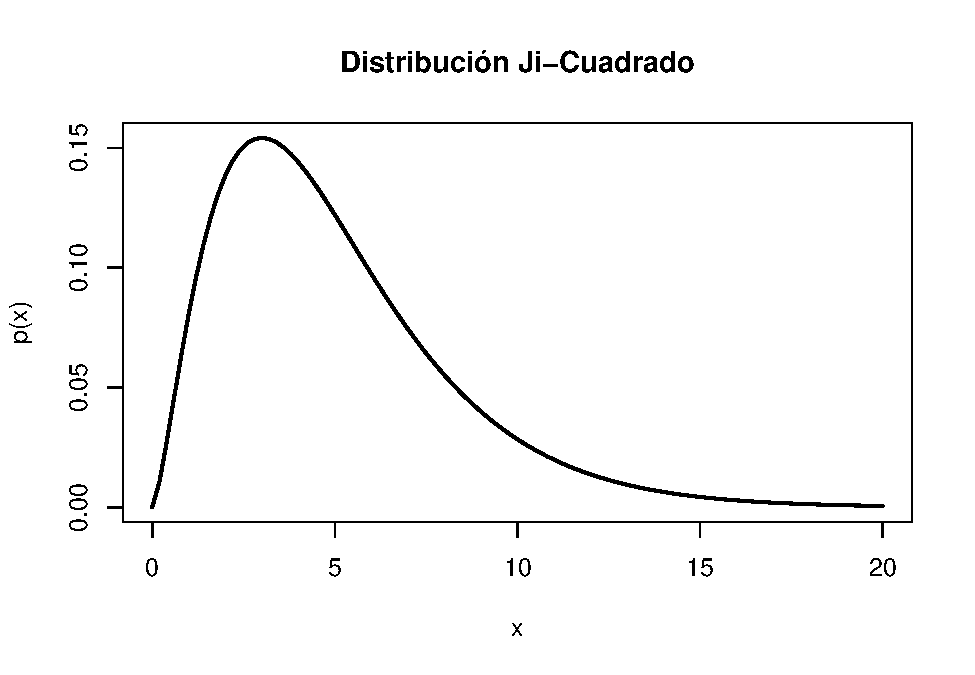
\includegraphics{NotaDeClaseLong_files/figure-latex/unnamed-chunk-18-2.pdf}

\begin{Shaded}
\begin{Highlighting}[]
  \CommentTok{#Graficando la región crítica}
  
  \CommentTok{#Selección de grados de libertad}
\NormalTok{  df <-}\StringTok{ }\DecValTok{6}
  \CommentTok{#Selección de error tipo I}
\NormalTok{  alpha <-}\StringTok{ }\FloatTok{0.10}
  \CommentTok{#Defino valor del eje de las abcisas (será un valor del estadístico) a partir del cual rechazo H0 }
\NormalTok{  rc <-}\StringTok{ }\KeywordTok{qchisq}\NormalTok{(}\DecValTok{1} \OperatorTok{-}\StringTok{ }\NormalTok{alpha, df)}
  
  \CommentTok{#Lo que haremos para graficar la región crítica será construir un polígono con la forma de la distribución}
  
  \CommentTok{#Defino el eje x (técnicamente debería seguir hasta infinito, pero a fines del gráfico se corta antes)}
\NormalTok{  x <-}\StringTok{ }\KeywordTok{seq}\NormalTok{(}\DecValTok{0}\NormalTok{,}\DecValTok{30}\NormalTok{,}\FloatTok{0.01}\NormalTok{)}
  \CommentTok{#Defino la región crítica en el eje}
\NormalTok{  z <-}\StringTok{ }\KeywordTok{seq}\NormalTok{(rc,}\DecValTok{30}\NormalTok{,}\FloatTok{0.01}\NormalTok{)}
  \CommentTok{#Defino el "lado" suoerior del polígono, que será una curva con la forma de la distribución en el segmento que quiero}
\NormalTok{  p <-}\StringTok{ }\KeywordTok{dchisq}\NormalTok{(z, df)}
  \CommentTok{#redefino los vectores de lados para la función polígono }
\NormalTok{  z <-}\StringTok{ }\KeywordTok{c}\NormalTok{(z,}\DecValTok{30}\NormalTok{,rc)}
\NormalTok{  p <-}\StringTok{ }\KeywordTok{c}\NormalTok{(p,}\KeywordTok{min}\NormalTok{(p),}\KeywordTok{min}\NormalTok{(p))}
  
  \CommentTok{#Grafico distribución Ji-Cuadrado}
  \KeywordTok{plot}\NormalTok{(x,}\KeywordTok{dchisq}\NormalTok{(x, df),}\DataTypeTok{type=}\StringTok{"l"}\NormalTok{,}
       \DataTypeTok{ylab=}\StringTok{"p(x)"}\NormalTok{,}\DataTypeTok{xlab=}\StringTok{"x"}\NormalTok{, }
       \DataTypeTok{ylim=}\KeywordTok{c}\NormalTok{(}\FloatTok{0.005}\NormalTok{,}\FloatTok{0.15}\NormalTok{), }\DataTypeTok{xlim =} \KeywordTok{c}\NormalTok{(}\DecValTok{0}\NormalTok{,}\DecValTok{25}\NormalTok{),}
       \DataTypeTok{main =} \StringTok{"Región Crítica del test Ji-Cuadrado"}\NormalTok{) }
  \CommentTok{#ylim sólo está para que quede el eje x bien cruzado con el cero}
  \CommentTok{#Agrego al gráfico el polígono}
  \KeywordTok{polygon}\NormalTok{(z,p,}\DataTypeTok{col=}\StringTok{"gray45"}\NormalTok{)}
  \CommentTok{#Agrego una línea que define la región crítica}
  \KeywordTok{segments}\NormalTok{(}\DataTypeTok{x0=}\NormalTok{rc, }\DataTypeTok{y0=}\DecValTok{0}\NormalTok{, }\DataTypeTok{x1=}\DecValTok{30}\NormalTok{, }\DataTypeTok{y1=}\DecValTok{0}\NormalTok{, }\DataTypeTok{lwd=}\DecValTok{3}\NormalTok{)}
    \KeywordTok{legend}\NormalTok{(}\StringTok{'center'}\NormalTok{,}
         \KeywordTok{expression}\NormalTok{(gl}\OperatorTok{==}\DecValTok{6}\NormalTok{, alpha}\OperatorTok{==}\FloatTok{0.10}\NormalTok{),}
         \DataTypeTok{bty =} \StringTok{"n"}\NormalTok{)}
\end{Highlighting}
\end{Shaded}

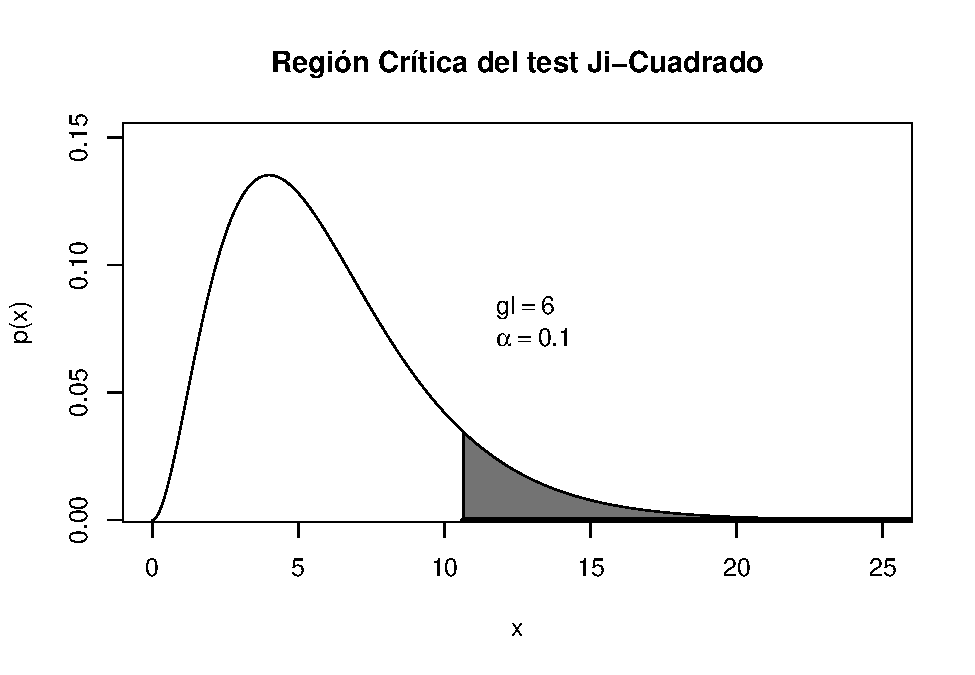
\includegraphics{NotaDeClaseLong_files/figure-latex/unnamed-chunk-18-3.pdf}

Hablar del \(R^2\)? QQ plots? Jarque Bera?

\hypertarget{inferencia-bayesiana}{%
\section{Inferencia Bayesiana}\label{inferencia-bayesiana}}


\end{document}
